\documentclass[10pt,answers]{exam}
\usepackage[spanish]{babel}
\usepackage[utf8]{inputenc}
\usepackage[T1]{fontenc}
\usepackage{amsmath,amssymb,amsfonts}
\usepackage{graphicx}
\usepackage{colortbl}
\usepackage{xcolor}
\usepackage{multirow}
\usepackage{float}
\usepackage{enumitem}
\usepackage{algorithm}
\usepackage{mathrsfs}
\usepackage{array} % Para controlar el ancho de las celdas
\usepackage{enumitem} % Para personalizar listas
\usepackage{listings}% http://ctan.org/pkg/listings
\usepackage{hyperref} % for hyperlinks
\usepackage{amsmath} % para matemáticas mejoradas
\usepackage{algorithm} % para escribir pseudocódigos
\usepackage{algpseudocode} % para escribir pseudocódigos
\usepackage[version=4]{mhchem}
\usepackage{stmaryrd}

% \usepackage{etoolbox}

% \AtBeginEnvironment{align}{\setcounter{equation}{0}}

\renewcommand{\solutiontitle}{\noindent\textbf{Solución:}\par\noindent}

\lstset{
  basicstyle=\ttfamily,
  mathescape
}

\graphicspath{{public/}}

\setlength{\topmargin}{-.5in} \setlength{\textheight}{9.25in}
\setlength{\oddsidemargin}{-0.5in} \setlength{\textwidth}{7.2in}


\begin{document}
\begin{center}
    \newcommand{\HRule}{\rule{\linewidth}{0.5mm}}
    \begin{minipage}{0.48\textwidth} 
        \begin{flushleft}
            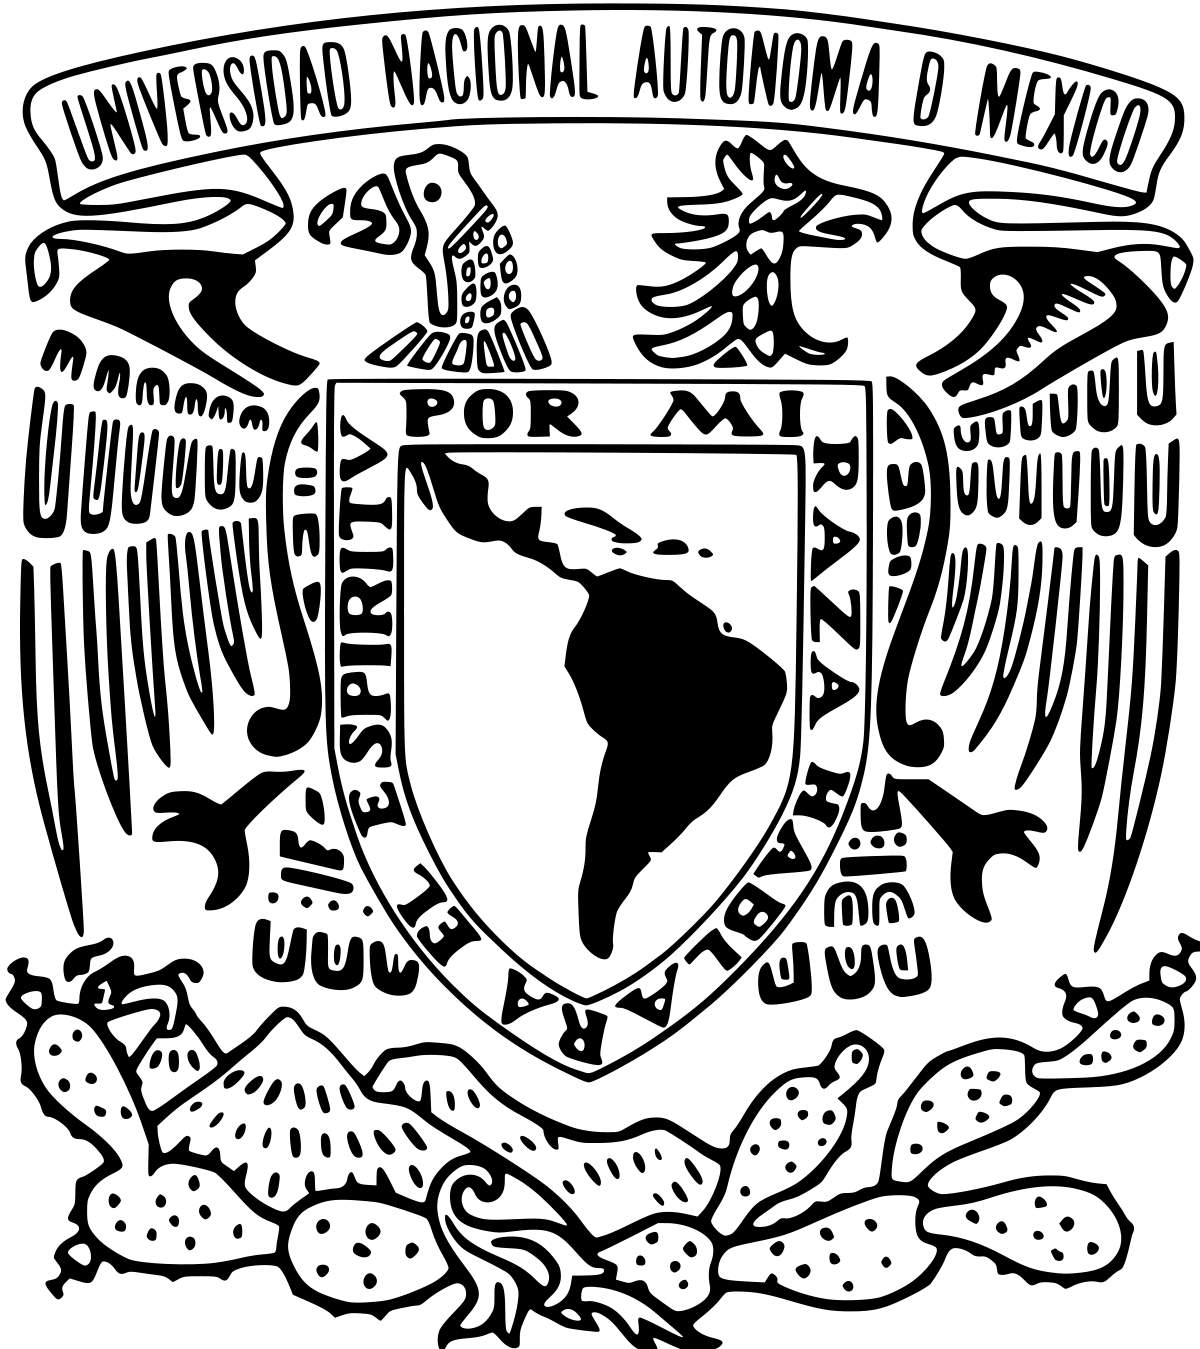
\includegraphics[scale = 0.08]{../../../public/logo_unam.png}
        \end{flushleft}
    \end{minipage}
    \begin{minipage}{0.48\textwidth} 
        \begin{flushright}
            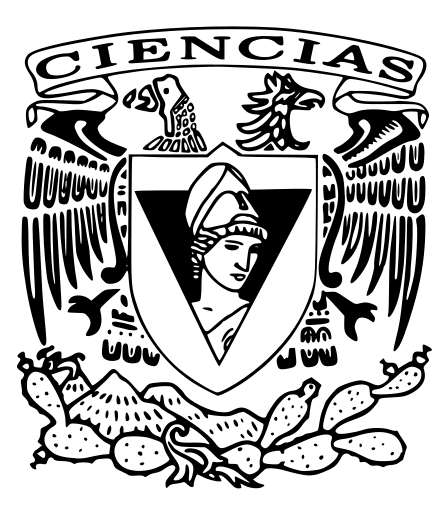
\includegraphics[scale =0.22]{../../../public/logo_ciencias.png}
        \end{flushright}
    \end{minipage}
    \vspace*{-1.5cm}						
    \textsc{\huge Nacional Autónoma de México \\ \vspace{-4px} Universidad }\\[2cm]	
    \textsc{\LARGE Facultad de Ciencias}\\[1.5cm]
    \vspace*{1cm}					
        \HRule \\[0.7cm]							
            { \huge \bfseries Tarea 03}\\[0.4cm]	
        \HRule \\[1.5cm]						    
    \begin{minipage}{0.52\textwidth}													
        \begin{flushleft} \large	
            \small
            \vspace{-0.6cm}	
            \vspace{-0.6cm}	
                \emph{Alumno:}\\
               Ramírez López Alvaro. 316276355\\
            \vspace*{2cm}
        \end{flushleft}																		
        \end{minipage}		
    \begin{minipage}{0.46\textwidth}		
        \vspace{-0.6cm}											
        \begin{flushright} \large						
            \small										
            \emph{Profesor:} Jesús Villagómez Chávez	\\
            \emph{Ayudantes:}
                Gabriela Peña Franco	 \\
                Martha Rubí Gutiérrez González	 \\
        \end{flushright}																
    \end{minipage}	
    \vspace*{1cm}
    \vspace{2cm}
    \begin{center}						
        {\large 9 de septiembre de 2024}
    \end{center}  						
\end{center}	
\textbf{}
\newpage

\begin{enumerate}

    \item ¿Cuáles de las siguientes relaciones son funciones? En caso de ser función, calcula su dominio y su imagen:
    \begin{enumerate}
        \item $\{(n,m) \in \mathbb{Z} \times \mathbb{Z} : n, m \geq 0 \land 5n = m\}$.
        \item $\{(n,m) \in \mathbb{Z} \times \mathbb{Z} : n, m \geq 0 \land 5m = n\}$.
        \item $\{(n,m) \in \mathbb{Z} \times \mathbb{Z} : n, m \geq 0 \land m \leq n\}$.
        \item $\{(n,m) \in \mathbb{Z} \times \mathbb{Z} : n \geq 0 \land m = 3\}$.
        \item $\{(n,m) \in \mathbb{Z} \times \mathbb{Z} : m = n^2\}$.
        \item $\{(n,m) \in \mathbb{Z} \times \mathbb{Z} : m^2 = n^2\}$.
        \item $\{(n,m) \in \mathbb{Z} \times \mathbb{Z} : 4n + 2m = 6\}$.
    \end{enumerate}

    \begin{solution}
\begin{enumerate}
    \item \(\{(n, m) \in \mathbb{Z} \times \mathbb{Z} \mid n, m \geq 0 \ \text{y} \ 5n = m\}\)

    \textbf{Análisis:} Para cada \( n \geq 0 \), existe un único \( m \geq 0 \) dado por \( m = 5n \).
    
    \textbf{Conclusión:} Es una función.
    
    \begin{itemize}
        \item Dominio: \( \{ n \in \mathbb{Z} \mid n \geq 0 \} \)
        \item Imagen: \( \{ m \in \mathbb{Z} \mid m = 5n, \ n \geq 0 \} = \{0, 5, 10, 15, \dots\} \)
    \end{itemize}
    
    \item \(\{(n, m) \in \mathbb{Z} \times \mathbb{Z} \mid n, m \geq 0 \ \text{y} \ 5m = n\}\)
    
    \textbf{Análisis:} Solo los \( n \geq 0 \) múltiplos de 5 tienen un \( m \geq 0 \) correspondiente dado por \( m = \frac{n}{5} \).
    
    \textbf{Conclusión:} Es una función, pero su dominio está restringido.
    
    \begin{itemize}
        \item Dominio:\( \{ n \in \mathbb{Z} \mid n \geq 0 \ \text{y} \ n \ \text{es múltiplo de} \ 5 \} \)
        \item Imagen: \( \{ m \in \mathbb{Z} \mid m \geq 0 \} \)
    \end{itemize}
    
    \item \(\{(n, m) \in \mathbb{Z} \times \mathbb{Z} \mid n, m \geq 0 \ \text{y} \ m \leq n\}\)

    \textbf{Análisis:} Para cada \( n \geq 0 \), existen múltiples valores de \( m \) que satisfacen \( m \leq n \).
        
    \textbf{Conclusión:} No es una función (no hay unicidad de \( m \) para cada \( n \)).
    
    \item \(\{(n, m) \in \mathbb{Z} \times \mathbb{Z} \mid n \geq 0 \ \text{y} \ m = 3\}\)
    
    \textbf{Análisis:} Para cada \( n \geq 0 \), \( m \) es siempre 3.
    
    \textbf{Conclusión:} Es una función.
    
    \begin{itemize}
        \item Dominio: \( \{ n \in \mathbb{Z} \mid n \geq 0 \} \)
        \item Imagen: \( \{3\} \)
    \end{itemize}
    
    
    \item \(\{(n, m) \in \mathbb{Z} \times \mathbb{Z} \mid m = n^2\}\)
    
    \textbf{Análisis:} Para cada \( n \in \mathbb{Z} \), existe un único \( m \) dado por \( m = n^2 \).
    
    \textbf{Conclusión:} Es una función.
    
    \begin{itemize}
        \item Dominio: \( \mathbb{Z} \)
        \item Imagen: \( \{ m \in \mathbb{Z} \mid m \geq 0 \ \text{y} \ m \ \text{es un cuadrado perfecto} \} \)
    \end{itemize}
    
    \item \(\{(n, m) \in \mathbb{Z} \times \mathbb{Z} \mid m^2 = n^2\}\)
    
    \textbf{Análisis:} Para cada \( n \), hay dos posibles valores de \( m \): \( m = n \) y \( m = -n \).
    
    \textbf{Conclusión:} No es una función (no hay unicidad de \( m \) para cada \( n \)).
    
    \item \(\{(n, m) \in \mathbb{Z} \times \mathbb{Z} \mid 4n + 2m = 6\}\)
    
    \textbf{Análisis:} Despejando \( m \), obtenemos \( m = 3 - 2n \). Para cada \( n \in \mathbb{Z} \), existe un único \( m \).
    
    \textbf{Conclusión:} Es una función.
    
    \begin{itemize}
        \item Dominio: \( \mathbb{Z} \)
        \item Imagen: \( \{ m \in \mathbb{Z} \mid m = 3 - 2n, \ n \in \mathbb{Z} \} \), es decir, todos los números enteros impares.
    \end{itemize}
\end{enumerate}
\end{solution}
    \item Determina la inyectividad, suprayectividad y biyectividad de las siguientes funciones:
    \begin{enumerate}
        \item $f : \mathbb{N} \rightarrow \mathbb{N}, f(n) = 2n$.
        \item $f : \mathbb{N} \rightarrow \mathbb{N}, f(n) = n + 7$.
        \item $f : \mathbb{Z} \rightarrow \mathbb{Z}, f(n) = n + 7$.
        \item $f : A \rightarrow A/R, f(a) = [a]_R$, donde $A$ es un conjunto y $R$ una relación de equivalencia sobre $A$.
    \end{enumerate}
    \begin{solution}
	\begin{enumerate}
		\item \( f : \mathbb{N} \rightarrow \mathbb{N}, \quad f(n) = 2n \)
		      \begin{itemize}
			      \item \textbf{Inyectividad:}Una función es inyectiva si \( f(n_1) = f(n_2) \) implica \( n_1 = n_2 \).
			            Supongamos que \( f(n_1) = f(n_2) \):

			            \[2n_1 = 2n_2 \implies n_1 = n_2\]

			            Por lo tanto, \( f \) es inyectiva.

			      \item \textbf{Suprayectividad:} Una función es suprayectiva si para todo \( y \in \mathbb{N} \), existe \( n \in \mathbb{N} \) tal que \( f(n) = y \).

			            El codominio es \( \mathbb{N} \), pero la imagen de \( f \) es el conjunto de los números naturales pares \( \{0, 2, 4, 6, \dots\} \).

			            Hay números naturales impares que no son imagen de ningún elemento de \( \mathbb{N} \) bajo \( f \).

			            Por lo tanto, \( f \) no es suprayectiva.

			      \item \textbf{Biyectividad:} Como \( f \) es inyectiva pero no suprayectiva, \( f \) no es biyectiva.
		      \end{itemize}

		\item \( f : \mathbb{N} \rightarrow \mathbb{N}, \quad f(n) = n + 7 \)
		      \begin{itemize}
			      \item \textbf{Inyectividad:}

			            Supongamos que \( f(n_1) = f(n_2) \):

			            \[
				            n_1 + 7 = n_2 + 7 \implies n_1 = n_2
			            \]

			            Por lo tanto, \( f \) es inyectiva.

			      \item \textbf{Suprayectividad:}

			            La imagen de \( f \) es \( \{ n + 7 \mid n \in \mathbb{N} \} \). El menor valor es \( f(0) = 7 \) (si consideramos \( \mathbb{N} = \{0, 1, 2, \dots\} \)).

			            Los números naturales menores que 7 no son imagen de ningún \( n \in \mathbb{N} \).

			            Por lo tanto, \( f \) no es suprayectiva.

			      \item \textbf{Biyectividad:} Como \( f \) es inyectiva pero no suprayectiva, \( f \) no es biyectiva.
		      \end{itemize}

		\item  \( f : \mathbb{Z} \rightarrow \mathbb{Z}, \quad f(n) = n + 7 \)
		      \begin{itemize}
			      \item \textbf{Inyectividad:}

			            Si \( f(n_1) = f(n_2) \):

			            \[
				            n_1 + 7 = n_2 + 7 \implies n_1 = n_2
			            \]

			            Por lo tanto, \( f \) es inyectiva.

			      \item \textbf{Suprayectividad:}

			            Para cualquier \( y \in \mathbb{Z} \), podemos encontrar \( n = y - 7 \in \mathbb{Z} \) tal que:

			            \[
				            f(n) = (y - 7) + 7 = y
				            \,           \]

			            Por lo tanto, \( f \) es suprayectiva.

			      \item \textbf{Biyectividad:} Como \( f \) es inyectiva y suprayectiva, \( f \) es biyectiva.
		      \end{itemize}

		\item  \( f : A \rightarrow A/R, \quad f(a) = [a]_R \)

		      Donde \( A \) es un conjunto y \( R \) es una relación de equivalencia sobre \( A \).

		      \begin{itemize}
			      \item \textbf{Inyectividad:}

			            La función \( f \) asigna a cada elemento \( a \in A \) su clase de equivalencia \( [a]_R \).

			            Si \( f(a_1) = f(a_2) \), entonces:

			            \[
				            [a_1]_R = [a_2]_R \implies a_1 \sim a_2
			            \]

			            Esto significa que \( a_1 \) y \( a_2 \) son equivalentes bajo \( R \), pero no necesariamente iguales.

			            Por lo tanto, \( f \) no es inyectiva a menos que \( R \) sea la relación de igualdad.

			      \item \textbf{Suprayectividad:}

			            Cada clase de equivalencia \( [a]_R \in A/R \) tiene al menos un representante en \( A \).

			            Por definición, para cualquier \( [a]_R \in A/R \), existe \( a \in A \) tal que \( f(a) = [a]_R \).

			            Por lo tanto, \( f \) es suprayectiva.

			      \item \textbf{Biyectividad:} Como \( f \) es suprayectiva pero no inyectiva, \( f \) no es biyectiva.
		      \end{itemize}
	\end{enumerate}
\end{solution}

    \item Sea $f : A \rightarrow B$ una función. Demuestra que:
    \begin{enumerate}
        \item $f$ es inyectiva si y sólo si $f^{-1}[f[X]] = X$, para todo $X \subseteq A$.
        \item $f$ es inyectiva si y sólo si $f[X \cap Y] = f[X] \cap f[Y]$, para $X, Y \subseteq A$.
        \item $f$ es suprayectiva si y sólo si $f[f^{-1}[Y]] = Y$, para todo $Y \subseteq B$.
        \item $f$ es biyectiva si y sólo si $f[X^c] = (f[X])^c$, para todo $X \subseteq A$.
    \end{enumerate}
    \begin{solution}
   \begin{enumerate}
    \item \( f \) es inyectiva si y sólo si \( f^{-1}[f[X]] = X \) para todo \( X \subseteq A \).**
    
    \textbf{Demostración:}
    
    ($\Rightarrow$) Si \( f \) es inyectiva, entonces \( f^{-1}[f[X]] = X \) para todo \( X \subseteq A \).
    
    Sea \( X \subseteq A \). Queremos demostrar que \( f^{-1}[f[X]] = X \).
    
    Primero, probamos que \( X \subseteq f^{-1}[f[X]] \):
    
    Esto es siempre cierto, independientemente de si \( f \) es inyectiva o no.
    
    Sea \( x \in X \). Entonces, \( f(x) \in f[X] \).
    
    Por definición de preimagen:
    
    \[x \in f^{-1}[f[X]] \quad \text{porque} \quad f(x) \in f[X].\]
    
    Por lo tanto, \( x \in f^{-1}[f[X]] \), y así \( X \subseteq f^{-1}[f[X]] \).
    
    Ahora, probamos que \( f^{-1}[f[X]] \subseteq X \):
    
    Supongamos que \( y \in f^{-1}[f[X]] \). Entonces, \( f(y) \in f[X] \).
    
    Esto significa que existe \( x \in X \) tal que \( f(y) = f(x) \).
    
    Como \( f \) es inyectiva y \( f(y) = f(x) \), entonces \( y = x \).
    
    Pero \( x \in X \), por lo que \( y \in X \).
    
    Por lo tanto, \( f^{-1}[f[X]] \subseteq X \).
    
    \textbf{Conclusión:}
    
    Combinando ambos resultados, obtenemos \( f^{-1}[f[X]] = X \).
    
    ($\Leftarrow$) Si \( f^{-1}[f[X]] = X \) para todo \( X \subseteq A \), entonces \( f \) es inyectiva.
    
    Supongamos que \( f \) no es inyectiva. Entonces, existen \( a_1, a_2 \in A \) con \( a_1 \neq a_2 \) tales que \( f(a_1) = f(a_2) \).
    
    Sea \( X = \{ a_1 \} \).
    
    Entonces, \( f[X] = \{ f(a_1) \} \).
    
    Ahora, calculemos \( f^{-1}[f[X]] \):
    
    \[f^{-1}[f[X]] = f^{-1}[\{ f(a_1) \}] = \{ x \in A \mid f(x) = f(a_1) \}.\]
    
    Pero sabemos que tanto \( a_1 \) como \( a_2 \) están en \( f^{-1}[f[X]] \) porque \( f(a_1) = f(a_2) \).
    
    Por lo tanto:
    \[f^{-1}[f[X]] \supseteq \{ a_1, a_2 \}.\]
    
    Pero \( X = \{ a_1 \} \), entonces \( f^{-1}[f[X]] \neq X \).
    
    Esto contradice la suposición de que \( f^{-1}[f[X]] = X \) para todo \( X \subseteq A \).
    
    \textbf{Conclusión:}
    
    Por contraposición, si \( f^{-1}[f[X]] = X \) para todo \( X \subseteq A \), entonces \( f \) es inyectiva.
    
    \item \( f \) es inyectiva si y sólo si \( f[X \cap Y] = f[X] \cap f[Y] \) para todo \( X, Y \subseteq A \).
    
    ($\Rightarrow$) Si \( f \) es inyectiva, entonces \( f[X \cap Y] = f[X] \cap f[Y] \).
    
    \textbf{Prueba:}
    
    Primero, probamos que \( f[X \cap Y] \subseteq f[X] \cap f[Y] \):
    
    Sea \( y \in f[X \cap Y] \). Entonces, existe \( x \in X \cap Y \) tal que \( y = f(x) \).
    
    Como \( x \in X \) y \( x \in Y \), entonces \( y \in f[X] \) y \( y \in f[Y] \).
    
    Por lo tanto, \( y \in f[X] \cap f[Y] \).
    
    Ahora, probamos que \( f[X] \cap f[Y] \subseteq f[X \cap Y] \):
    
    Sea \( y \in f[X] \cap f[Y] \). Entonces, existe \( x_1 \in X \) tal que \( y = f(x_1) \) y existe \( x_2 \in Y \) tal que \( y = f(x_2) \).
    
    Como \( f \) es inyectiva y \( f(x_1) = f(x_2) \), entonces \( x_1 = x_2 \).
    
    Por lo tanto, \( x_1 \in X \cap Y \), y así \( y = f(x_1) \in f[X \cap Y] \).
    
    \textbf{Conclusión:}
    
      Por ambos resultados, \( f[X \cap Y] = f[X] \cap f[Y] \).
    
    ($\Leftarrow$) Si \( f[X \cap Y] = f[X] \cap f[Y] \) para todo \( X, Y \subseteq A \), entonces \( f \) es inyectiva.
    
    \textbf{Prueba:}
    
    Supongamos que \( f \) no es inyectiva. Entonces, existen \( a_1, a_2 \in A \) con \( a_1 \neq a_2 \) tales que \( f(a_1) = f(a_2) \).
    
    Sea \( X = \{ a_1 \} \) y \( Y = \{ a_2 \} \).
    
    Entonces:
    
    \( X \cap Y = \emptyset \), por lo que \( f[X \cap Y] = f[\emptyset] = \emptyset \).

    \( f[X] = \{ f(a_1) \} \).

    \( f[Y] = \{ f(a_2) \} \).

    Como \( f(a_1) = f(a_2) \), entonces \( f[X] = f[Y] = \{ f(a_1) \} \).
    
    Por lo tanto, \( f[X] \cap f[Y] = \{ f(a_1) \} \).
    
    Pero entonces:
    
    \[f[X \cap Y] = \emptyset \neq \{ f(a_1) \} = f[X] \cap f[Y].\]
    
    Esto contradice la suposición de que \( f[X \cap Y] = f[X] \cap f[Y] \).
    
    \textbf{Conclusión:}
    
    Por contraposición, si \( f[X \cap Y] = f[X] \cap f[Y] \) para todo \( X, Y \subseteq A \), entonces \( f \) es inyectiva.
    
    \item \( f \) es suprayectiva si y sólo si \( f[f^{-1}[Y]] = Y \) para todo \( Y \subseteq B \).
    
    \textbf{Demostración:}
    
    **($\Rightarrow$) Si \( f \) es suprayectiva, entonces \( f[f^{-1}[Y]] = Y \) para todo \( Y \subseteq B \).**
    
    \textbf{Prueba:}
    
    Sea \( Y \subseteq B \).
    
    Primero, probamos que \( f[f^{-1}[Y]] \subseteq Y \):
    
    Sea \( y \in f[f^{-1}[Y]] \). Entonces, existe \( x \in f^{-1}[Y] \) tal que \( y = f(x) \).
    
    Por definición de \( f^{-1}[Y] \), tenemos \( f(x) \in Y \).
    
    Entonces, \( y = f(x) \in Y \).
    
    Por lo tanto, \( f[f^{-1}[Y]] \subseteq Y \).
    
    Ahora, probamos que \( Y \subseteq f[f^{-1}[Y]] \):
    
    Sea \( y \in Y \).
    
    Como \( f \) es suprayectiva, existe \( x \in A \) tal que \( f(x) = y \).
    
    Por lo tanto, \( x \in f^{-1}[Y] \) porque \( f(x) = y \in Y \).
    
    Entonces, \( y = f(x) \in f[f^{-1}[Y]] \).
    
    Por lo tanto, \( Y \subseteq f[f^{-1}[Y]] \).
    
    \textbf{Conclusión:}
    
    Combinando ambos resultados, \( f[f^{-1}[Y]] = Y \).
    
    ($\Leftarrow$) Si \( f[f^{-1}[Y]] = Y \) para todo \( Y \subseteq B \), entonces \( f \) es suprayectiva.
    
    \textbf{Prueba:}
    
    Supongamos que \( f \) no es suprayectiva. Entonces, existe \( b_0 \in B \) tal que no existe \( a \in A \) con \( f(a) = b_0 \).
    
    Sea \( Y = \{ b_0 \} \).
    
    Entonces, \( f^{-1}[Y] = \emptyset \) porque no hay ningún \( a \in A \) tal que \( f(a) = b_0 \).
    
    Por lo tanto:
    
    \[f[f^{-1}[Y]] = f[\emptyset] = \emptyset \neq Y = \{ b_0 \}.\]
    
    Esto contradice la suposición de que \( f[f^{-1}[Y]] = Y \) para todo \( Y \subseteq B \).
    
    \textbf{Conclusión:}
    
    Por contraposición, si \( f[f^{-1}[Y]] = Y \) para todo \( Y \subseteq B \), entonces \( f \) es suprayectiva.
    
    \item \( f \) es biyectiva si y sólo si \( f[X^c] = (f[X])^c \) para todo \( X \subseteq A \).
    
    \textbf{Demostración:}
    
    Primero, recordemos que:
    
    \( X^c = A \setminus X \), el complemento de \( X \) en \( A \).

    \( (f[X])^c = B \setminus f[X] \), el complemento de \( f[X] \) en \( B \).
    
    ($\Rightarrow$) Si \( f \) es biyectiva, entonces \( f[X^c] = (f[X])^c \) para todo \( X \subseteq A \).
    
    \textbf{Prueba:}
    
    Sea \( X \subseteq A \).
    
    Primero, probamos que \( f[X^c] \subseteq (f[X])^c \):
    
    Sea \( y \in f[X^c] \). Entonces, existe \( x \in X^c \) tal que \( y = f(x) \).
    
    Si \( y \in f[X] \), entonces existiría \( x' \in X \) tal que \( y = f(x') \).
    
    Pero como \( f \) es inyectiva (por ser biyectiva), \( x = x' \), lo cual es imposible porque \( x \in X^c \) y \( x' \in X \).
    
    Por lo tanto, \( y \notin f[X] \), y así \( y \in (f[X])^c \).
    
    Ahora, probamos que \( (f[X])^c \subseteq f[X^c] \):
    
    Sea \( y \in (f[X])^c \). Entonces, \( y \notin f[X] \).
    
    Como \( f \) es sobreyectiva, existe \( x \in A \) tal que \( f(x) = y \).
    
    Si \( x \in X \), entonces \( y = f(x) \in f[X] \), contradicción.
    
    Por lo tanto, \( x \in X^c \), y así \( y = f(x) \in f[X^c] \).
    
    \textbf{Conclusión:}
    
    Por ambos resultados, \( f[X^c] = (f[X])^c \).
    
    ($\Leftarrow$) Si \( f[X^c] = (f[X])^c \) para todo \( X \subseteq A \), entonces \( f \) es biyectiva.
    
    \textbf{Prueba de inyectividad:}
    
    Supongamos que \( f \) no es inyectiva. Entonces, existen \( a_1, a_2 \in A \) con \( a_1 \neq a_2 \) y \( f(a_1) = f(a_2) = y_0 \).
    
    Sea \( X = \{ a_1 \} \).
    
    Entonces:
    
    \( X^c = A \setminus \{ a_1 \} \).
    
    \( f[X] = \{ f(a_1) \} = \{ y_0 \} \).
    
    \( f[X^c] \) contiene al menos \( f(a_2) = y_0 \) porque \( a_2 \in X^c \).
    
      Por lo tanto, \( y_0 \in f[X^c] \).
    
      Pero entonces:
    
      \[
      y_0 \in f[X^c] \implies y_0 \in (f[X])^c \quad \text{(por la suposición)}.
      \]
    
      Sin embargo, \( y_0 \in f[X] \), por lo que \( y_0 \notin (f[X])^c \).
    
      Esto es una contradicción.
    
    \textbf{Prueba de sobreyectividad:}
    
    Supongamos que \( f \) no es sobreyectiva. Entonces, existe \( y_1 \in B \) tal que no existe \( a \in A \) con \( f(a) = y_1 \).
    
    Sea \( X = A \).
    
    Entonces:
    
    \( X^c = \emptyset \).

    \( f[X] = f[A] \subsetneq B \) (porque \( f \) no es sobreyectiva).
    
    \( f[X^c] = f[\emptyset] = \emptyset \).
    
    \( (f[X])^c = B \setminus f[A] \), que contiene al menos \( y_1 \).
    
    Por lo tanto, \( y_1 \in (f[X])^c \).
    
    Pero \( f[X^c] = \emptyset \), entonces \( (f[X])^c \neq f[X^c] \), contradiciendo la suposición.
    
    \textbf{Conclusión:}
    
    Por contradicción, \( f \) debe ser inyectiva y sobreyectiva, es decir, biyectiva.
  \end{enumerate}
\end{solution}

    \item Responde las siguientes preguntas:
    \begin{enumerate}
        \item ¿Existe $g : \mathbb{N} \rightarrow \mathbb{N}$ función tal que $g \neq \text{Id}_{\mathbb{N}}$ y $g \circ g = g$?
        \item ¿Existe $g : \mathbb{N} \rightarrow \mathbb{N}$ función biyectiva tal que $g \neq \text{Id}_{\mathbb{N}}$ y $g \circ g = g$?
        \item ¿Existe $g : \mathbb{N} \rightarrow \mathbb{N}$ función biyectiva tal que $g \neq \text{Id}_{\mathbb{N}}$ y $g \circ g = \text{Id}_{\mathbb{N}}$?
    \end{enumerate}
    \begin{solution}
    \begin{enumerate}
      \item ¿Existe \( g : \mathbb{N} \rightarrow \mathbb{N} \) tal que \( g \neq \text{Id}_{\mathbb{N}} \) y \( g \circ g = g \)?
      
      Respuesta: Sí, existe tal función.
      
      \textbf{Explicación:}
      
      Una función que satisface \( g \circ g = g \) se denomina idempotente. Queremos encontrar una función idempotente que no sea la identidad.
      
      \textbf{Ejemplo de función:}
      
      Definamos \( g : \mathbb{N} \rightarrow \mathbb{N} \) como:
      
      \[
      g(n) = \begin{cases}
      0, & \text{si } n \text{ es impar} \\
      n, & \text{si } n \text{ es par}
      \end{cases}
      \]
      
      \textbf{Verificación:}
      
      \( g \neq \text{Id}_{\mathbb{N}} \): Porque \( g(n) \) cambia los números impares a 0, por lo que no es la función identidad.
        
      Idempotencia (\( g \circ g = g \)):
      
      Para todo \( n \in \mathbb{N} \):
      
      Si \( n \) es par:
          \[
          g(g(n)) = g(n) = n
          \]

      Si \( n \) es impar:
          \[
          g(g(n)) = g(0) = g(0) = 0 = g(n)
          \]
      
      En ambos casos, \( g(g(n)) = g(n) \), por lo que \( g \circ g = g \).
      
      \textbf{Conclusión:} Existe al menos una función \( g \) que cumple las condiciones dadas.
      
      \item ¿Existe \( g : \mathbb{N} \rightarrow \mathbb{N} \) biyectiva tal que \( g \neq \text{Id}_{\mathbb{N}} \) y \( g \circ g = g \)?
      
      \textbf{Respuesta:} No, no existe tal función.
      
      \textbf{Explicación:}
      
      Supongamos que existe una función biyectiva \( g : \mathbb{N} \rightarrow \mathbb{N} \) tal que \( g \circ g = g \) y \( g \neq \text{Id}_{\mathbb{N}} \).
      
      \textbf{Demostración por contradicción:}
      
      \( g \) es biyectiva, por lo que tiene una función inversa \( g^{-1} \).
      
      Dado que \( g \circ g = g \), podemos aplicar \( g^{-1} \) a ambos lados:
      
        \[
        g^{-1} \circ g \circ g = g^{-1} \circ g
        \]
      
      Simplificando:
      
        \[
        g \circ g^{-1} \circ g = \text{Id}_{\mathbb{N}} \circ g = g
        \]
      
      Pero dado que \( g^{-1} \circ g = \text{Id}_{\mathbb{N}} \), tenemos:
      
        \[
        \text{Id}_{\mathbb{N}} \circ g = g
        \]
      
      Esto implica que \( g = g \), lo cual es siempre cierto. Sin embargo, no hemos llegado a una contradicción aún.
      
      Consideremos que \( g \) es idempotente y biyectiva. La única función biyectiva idempotente es la identidad. Esto se debe a que si \( g \) es idempotente (\( g \circ g = g \)) y biyectiva, entonces para todo \( n \in \mathbb{N} \):
      
        \[
        g(n) = g(g(n))
        \]
      
      Como \( g \) es inyectiva, esto implica que:
      
        \[
        n = g(n)
        \]
      
      Por lo tanto, \( g \) es la identidad, lo cual contradice \( g \neq \text{Id}_{\mathbb{N}} \).
      
      Conclusión: No existe una función biyectiva \( g \) distinta de la identidad que sea idempotente.
      
      \item ¿Existe \( g : \mathbb{N} \rightarrow \mathbb{N} \) biyectiva tal que \( g \neq \text{Id}_{\mathbb{N}} \) y \( g \circ g = \text{Id}_{\mathbb{N}} \)?
      
      \textbf{Respuesta:} Sí, existe tal función.
      
      \textbf{Explicación:}
      
      Una función que satisface \( g \circ g = \text{Id}_{\mathbb{N}} \) se denomina involutiva. Queremos encontrar una función biyectiva involutiva que no sea la identidad.
      
      \textbf{Ejemplo de función:}
      
      Definamos \( g : \mathbb{N} \rightarrow \mathbb{N} \) como sigue:
      
      \[
      g(n) = \begin{cases}
      n + 1, & \text{si } n \text{ es par} \\
      n - 1, & \text{si } n \text{ es impar}
      \end{cases}
      \]
      
      \textbf{Verificación:}
      
      \( g \) es biyectiva:
      
      \textbf{Inyectividad:} Supongamos que \( g(n_1) = g(n_2) \). Entonces:
      
      Si ambos \( n_1 \) y \( n_2 \) son pares:
      \[n_1 + 1 = n_2 + 1 \implies n_1 = n_2\]
      
      Si ambos son impares: 
      \[n_1 - 1 = n_2 - 1 \implies n_1 = n_2\]
      
      Si uno es par y otro impar, sus imágenes serán distintas, pues uno será \( n + 1 \) y otro \( n - 1 \).
      
      \textbf{Sobreyectividad:} Para cualquier \( m \in \mathbb{N} \):
      
      Si \( m \) es par, entonces \( m = g(m - 1) \) (porque \( m - 1 \) es impar).
      
      Si \( m \) es impar, entonces \( m = g(m + 1) \) (porque \( m + 1 \) es par).
      
      \( g \neq \text{Id}_{\mathbb{N}} \):
      
      Porque, por ejemplo, \( g(0) = 1 \neq 0 \).
      
      Involutividad (\( g \circ g = \text{Id}_{\mathbb{N}} \)):
      
      Para todo \( n \in \mathbb{N} \):
      
      \begin{itemize}
        \item Si \( n \) es par:
        
        \( g(n) = n + 1 \) (impar).
            
        \( g(g(n)) = g(n + 1) \).
        
        Como \( n + 1 \) es impar, entonces:
        
        \[g(n + 1) = (n + 1) - 1 = n\]
        
        \item Si \( n \) es impar:
        
        \( g(n) = n - 1 \) (par).
        
        \( g(g(n)) = g(n - 1) \).
        
        Como \( n - 1 \) es par, entonces:
        \[g(n - 1) = (n - 1) + 1 = n\]
      \end{itemize}
      
        En ambos casos, \( g(g(n)) = n \), por lo que \( g \circ g = \text{Id}_{\mathbb{N}} \).
      
      \textbf{Conclusión:} Existe una función biyectiva \( g \) distinta de la identidad que es involutiva.
    \end{enumerate}
\end{solution}

    \item (Extra) Sea $f : A \rightarrow B$ una función. Definimos la asignación $F : B \rightarrow A$ con regla de correspondencia $F(Y) = f^{-1}[Y]$. Demuestra que:
    \begin{enumerate}
        \item $F$ es función.
        \item Si $f$ es inyectiva, entonces $F$ es suprayectiva.
        \item Si $f$ es suprayectiva, entonces $F$ es inyectiva.
        \item Si $F$ es suprayectiva, entonces $f$ es inyectiva.
        \item Si $F$ es inyectiva, entonces $F$ es suprayectiva.
    \end{enumerate}
    \begin{solution}

    Sea \( f : A \rightarrow B \) una función. Definimos la asignación \( F : \mathcal{P}(B) \rightarrow \mathcal{P}(A) \) con regla de correspondencia \( F(Y) = f^{-1}[Y] \), donde \( \mathcal{P}(B) \) es el conjunto de las partes de \( B \).
    
    \begin{enumerate}
        \item \( F \) es función.
        
        \textbf{Demostración:}
        
        Para demostrar que \( F \) es una función de \( \mathcal{P}(B) \) en \( \mathcal{P}(A) \), debemos mostrar que para cada \( Y \subseteq B \), existe un único \( F(Y) \subseteq A \).
        
        Por la definición de \( F \), para cada \( Y \subseteq B \), se asigna el conjunto \( F(Y) = f^{-1}[Y] \), que es el conjunto de todos los elementos en \( A \) cuya imagen por \( f \) pertenece a \( Y \):
        
        \[
        f^{-1}[Y] = \{ a \in A \mid f(a) \in Y \}.
        \]
        
        Este conjunto está bien definido para cada \( Y \subseteq B \). Por lo tanto, \( F \) es una función de \( \mathcal{P}(B) \) en \( \mathcal{P}(A) \).
        
        \item 2. Si \( f \) es inyectiva, entonces \( F \) es sobreyectiva.
        
        \textbf{Demostración:}
        
        Supongamos que \( f \) es inyectiva. Queremos demostrar que \( F \) es sobreyectiva, es decir, que para todo \( X \subseteq A \), existe \( Y \subseteq B \) tal que \( F(Y) = X \).
        
        Sea \( X \subseteq A \). Definamos \( Y = f[X] \), es decir:
        
        \[
        Y = \{ f(a) \mid a \in X \}.
        \]
        
        Ahora, calculemos \( F(Y) \):
        
        \[
        F(Y) = f^{-1}[Y] = \{ a \in A \mid f(a) \in Y \}.
        \]
        
        Pero como \( Y = f[X] \), entonces \( f(a) \in Y \) si y solo si \( f(a) \in f[X] \). Dado que \( f \) es inyectiva, \( f(a) \in f[X] \) si y solo si \( a \in X \).
        
        Por lo tanto:
        
        \[
        F(Y) = \{ a \in A \mid a \in X \} = X.
        \]
        
        Así, para todo \( X \subseteq A \), existe \( Y = f[X] \subseteq B \) tal que \( F(Y) = X \).
        
        \textbf{Conclusión:} \( F \) es sobreyectiva.
        
        \item Si \( f \) es suprayectiva, entonces \( F \) es inyectiva.
        
        \textbf{Demostración:}
        
        Supongamos que \( f \) es suprayectiva. Queremos demostrar que \( F \) es inyectiva, es decir, que si \( F(Y_1) = F(Y_2) \) entonces \( Y_1 = Y_2 \).
        
        Sea \( Y_1, Y_2 \subseteq B \) tales que \( F(Y_1) = F(Y_2) \). Entonces:
        
        \[
        f^{-1}[Y_1] = f^{-1}[Y_2].
        \]
        
        Queremos demostrar que \( Y_1 = Y_2 \).
        
        Dado que \( f \) es suprayectiva, para todo \( y \in B \) existe \( a \in A \) tal que \( f(a) = y \).
        
        Ahora, tomemos \( y \in Y_1 \). Como \( f \) es suprayectiva, existe \( a \in A \) tal que \( f(a) = y \). Entonces, \( a \in f^{-1}[Y_1] \).
        
        Pero \( f^{-1}[Y_1] = f^{-1}[Y_2] \), por lo que \( a \in f^{-1}[Y_2] \), lo que implica que \( f(a) \in Y_2 \). Por lo tanto, \( y \in Y_2 \).
        
        De manera similar, si \( y \in Y_2 \), entonces \( y \in Y_1 \).
        
        Por lo tanto, \( Y_1 = Y_2 \).
        
        \textbf{Conclusión:} \( F \) es inyectiva.
        
        \item Si \( F \) es sobreyectiva, entonces \( f \) es inyectiva.
        
        \textbf{Demostración:}
        
        Supongamos que \( F \) es sobreyectiva y que \( f \) no es inyectiva. Buscaremos una contradicción.
        
        Como \( f \) no es inyectiva, existen \( a_1, a_2 \in A \) con \( a_1 \neq a_2 \) tales que \( f(a_1) = f(a_2) = b \).
        
        Consideremos el conjunto \( X = \{ a_1 \} \subseteq A \). Como \( F \) es sobreyectiva, existe \( Y \subseteq B \) tal que \( F(Y) = X \).
        
        Entonces, \( F(Y) = f^{-1}[Y] = \{ a \in A \mid f(a) \in Y \} = \{ a_1 \} \).
        
        Pero sabemos que \( f(a_1) = b \), por lo que \( a_1 \in f^{-1}[Y] \) implica que \( b = f(a_1) \in Y \).
        
        Del mismo modo, como \( f(a_2) = b \) y \( b \in Y \), entonces \( a_2 \in f^{-1}[Y] \).
        
        Esto significa que \( a_2 \in F(Y) = \{ a_1 \} \), lo cual es una contradicción, ya que \( a_2 \neq a_1 \).
        
        \textbf{Conclusión:} Nuestra suposición de que \( f \) no es inyectiva conduce a una contradicción. Por lo tanto, si \( F \) es sobreyectiva, entonces \( f \) es inyectiva.
        
        \item Si \( F \) es inyectiva, entonces \( F \) es sobreyectiva.
        
        \textbf{Demostración:}
        
        Supongamos que \( F \) es inyectiva. Queremos demostrar que \( F \) es sobreyectiva, es decir, que para todo \( X \subseteq A \), existe \( Y \subseteq B \) tal que \( F(Y) = X \).
        
        Sin embargo, en general, la inyectividad de \( F \) no implica que \( F \) sea sobreyectiva. Veamos un contraejemplo.
        
        \textbf{Contraejemplo:}
        
        Consideremos los conjuntos \( A = \{1\} \) y \( B = \{a, b\} \). Definamos \( f : A \rightarrow B \) como \( f(1) = a \).
        
        La función \( f \) es inyectiva (ya que \( A \) tiene un solo elemento), pero no es suprayectiva (ya que \( b \notin f(A) \)).
        
        Ahora, definamos \( F : \mathcal{P}(B) \rightarrow \mathcal{P}(A) \):
        
        \( F(\emptyset) = f^{-1}[\emptyset] = \emptyset \).
        
        \( F(\{a\}) = f^{-1}[\{a\}] = \{1\} \).
        
        \( F(\{b\}) = f^{-1}[\{b\}] = \emptyset \).
        
        \( F(\{a, b\}) = f^{-1}[\{a, b\}] = \{1\} \).
        
        Observamos que \( F(\{a\}) = F(\{a, b\}) = \{1\} \). Sin embargo, \( \{a\} \neq \{a, b\} \), lo que indica que \( F \) no es inyectiva, contradiciendo nuestra suposición.
        
        Pero este contraejemplo muestra que la inyectividad de \( F \) no garantiza su sobreyectividad. De hecho, en este ejemplo, \( F \) no es sobreyectiva (ya que no alcanza ciertos subconjuntos de \( \mathcal{P}(A) \)).
        
        \textbf{Conclusión:}
        
        La inyectividad de \( F \) no implica que \( F \) sea sobreyectiva. Por lo tanto, el enunciado es falso en general.
    \end{enumerate}
\end{solution}

\end{enumerate}

\end{document}